\chapter{OLAP Analysis on Graph Database}
In this chapter we will propose a system capable of executing OLAP analysis and that supports heterogeneous graphs, without the need to define a new graph data model. Initially, we will contextualise the proposed system and introduce a running example that will be used to better explain the system operation. Then, the system's architecture is presented and its main components are further detailed in the following sections.

\section{Contextualisation}

In Chapter 3, we investigated some of the main works in the area of Graph OLAP. Most of them only give support to homogeneous graphs \cite{Zhao2011}\cite{Chen2008}\cite{Wang2014}, while real world graph-like data contains different types of vertices and edges.The frameworks HMGraph \cite{Yin2012} and GRAD Graph Cube \cite{ghrab2015framework} support heterogeneous graphs, but they propose a new multidimensional model in order to do OLAP analysis.

The objective of the system proposed here is to support OLAP analysis on heterogeneous graph databases without the need to re-model operational data. This will be done by adding a layer of pre-processed aggregate graphs and an analytical query processor module on top of the operational graph database.

\section{Running Example}
Consider the Database System and Logic Programming (DBLP) dataset as the running example that will be used throughout this chapter to help explaining the main concepts of the system proposed. The DBLP\footnote{http://dblp.uni-trier.de/faq/What+is+dblp.html} is an online computer science bibliography that, up until May 2016, indexes more than 3.3 million publications by more than 1.7 million authors. For this example, we will consider that the data was extracted and modelled according to the schema shown in Figure \ref{fig:figure25} and described as follows:

\begin{itemize}
\item Each publication becomes a vertex with label \emph{Publication} and with the attributes \emph{title}, \emph{year} and \emph{venue}.
\item Each author becomes a vertex with label \emph{Author} and with the attribute \emph{name}
\item Edges labeled \emph{PUBLISHED} connect Author vertices to Publication vertices, representing the relationship between an author and their published work.
\item Edges labeled \emph{COAUTHOR} connect Author vertices to other Author vertices, representing the relationship between authors that have contributed to the same published work.
\end{itemize}

\begin{figure}[ht]
\centering
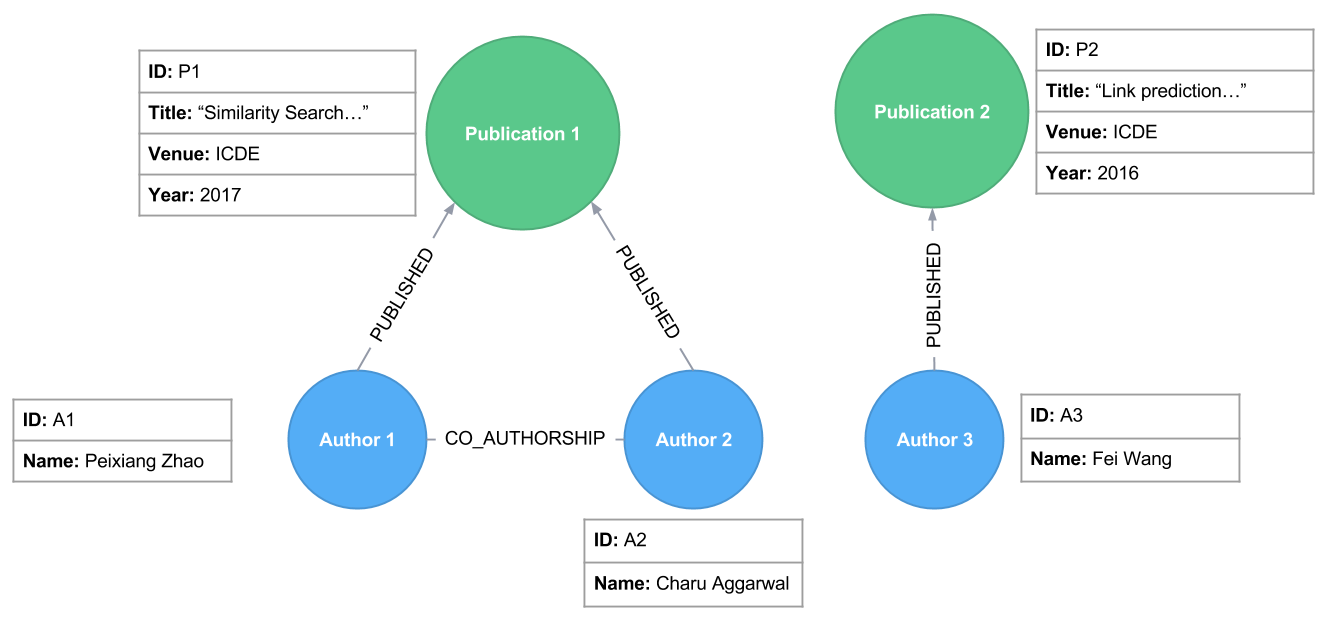
\includegraphics[width=0.8\textwidth]{../dblp_schema_with_attr.png}
\caption{Schema representation of the DBLP data graph}
\label{fig:figure25}
\end{figure}

Figure \ref{fig:figure26} shows a subset of the original DBLP dataset, modelled according to the schema representation depicted in Figure \ref{fig:figure25}. The following graph will be used as our running example throughout this chapter.

\begin{figure}[ht]
\centering
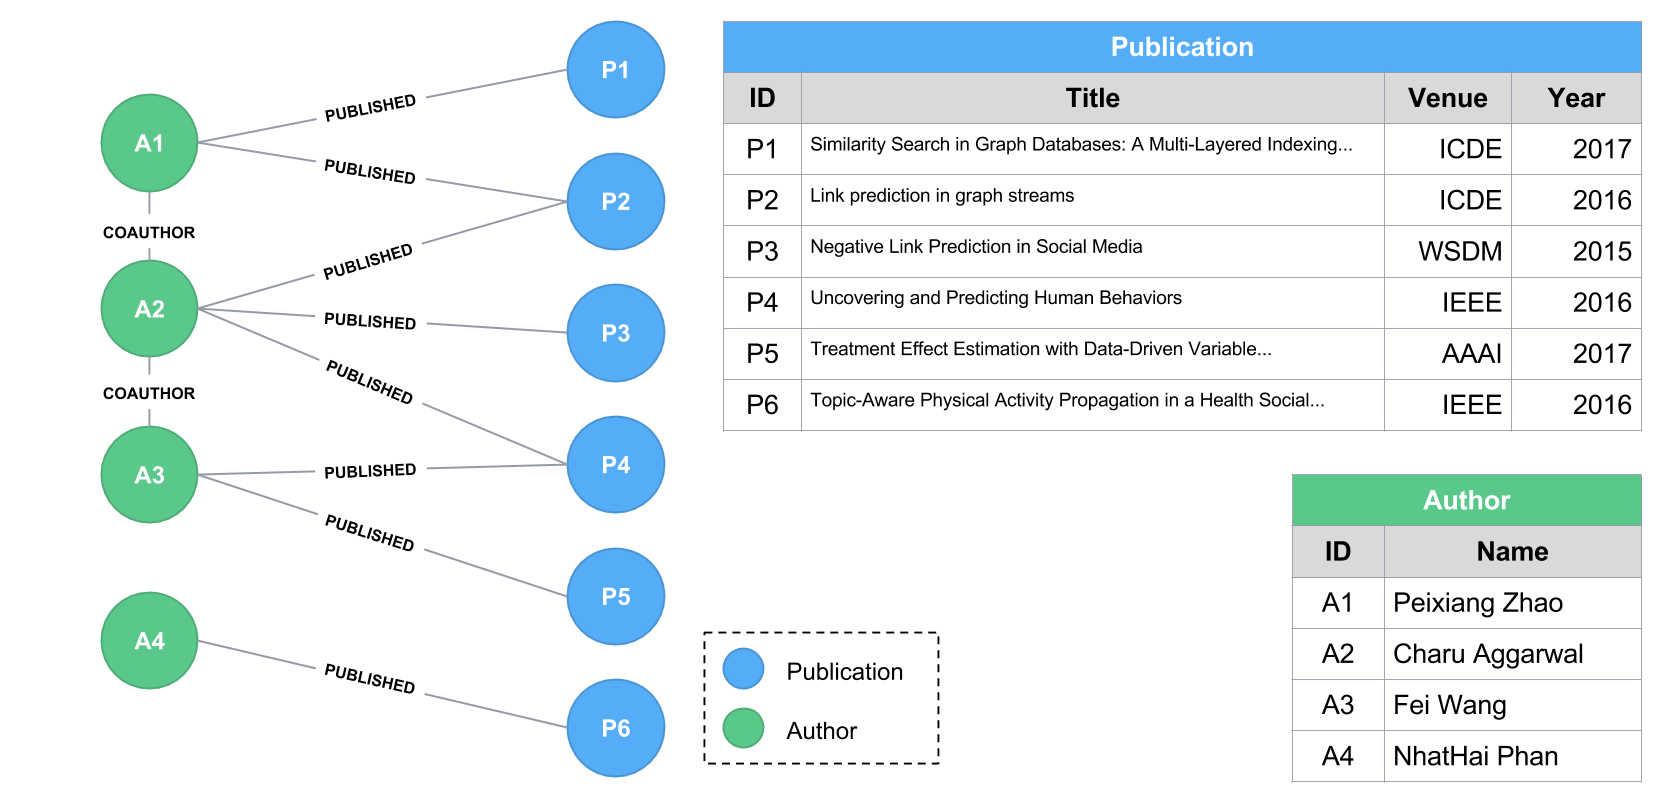
\includegraphics[width=1\textwidth]{../running_example.png}
\caption{Running Example with subset of DBLP dataset}
\label{fig:figure26}
\end{figure}

\section{Dimensions and Measures}

As discussed in Chapter 2, an OLAP system is a tool that facilitates multidimensional analysis of the data. In order to perform such kind of analysis, it is necessary to define the dimensions and measures that will be considered during the multidimensional analysis:
\begin{description}
\item[Dimension] Given a labeled property graph $G = (V, E, L_V, L_E, A_V, A_E)$, where:
\begin{itemize}
\item $V$ is a set of vertices
\item $E \subseteq V \times V$ is a set of edges 
\item $L_V$ is a set of vertices labels and $L_E$ is a set of edge labels
\item $A_V = \{a_1, \dots, a_n\}$ is a set of vertex attributes, where $a_i = (k_i, m_i)$ is a key-value pair, $k_i$ is the attribute key and $m_i$ is the attribute value. Each vertex $v_i \in V$ is associated with a set of attributes. $A_E = \{b_1, \dots, b_n\}$ is the set of edge attributes defined in the same way as vertex attributes.
\end{itemize}
 A dimension is given by $d = (a, l)$, where $a \in A_V$ and $l \in L_V$. 

In our running example, we can define $d_1 = (journal, Publication)$ and $d_2 = (year, Publication)$, i.e. the \emph{Publication} attributes \emph{journal} and \emph{year} are dimensions $d_1$ and $d_2$ in our OLAP system, respectively.

\item[Measure] Given a labeled property graph $G = (V, E, L_V, L_E, A_V, A_E)$, a measure $m$ is a calculation computed over the graph $G$ using a function $F$ ($m=F(G)$), that can return the type of measures defined by  \cite{ghrab2015framework}:
\begin{description}
\item[Content-based measure] For this kind of measure is calculated based on the vertices and edges attributes and the function $F \in \{SUM, COUNT, AVG, or other aggregate functions\}$ used in the calculation are similar to the ones used in an OLAP system. 

In our running example, the total number of authors that published a work in 2007 is a content-based measure that is calculated using the function $COUNT$, which will count the number of \emph{Author} vertices that have a relationship \emph{PUBLISHED} to \emph{Publication} vertices that have attribute \emph{year} equals to 2007.
\item[Graph-based measure] This type of measure is calculated by applying a network analysis algorithm over the graph, i.e. a network analysis algorithm is used as the function $F$. 

In our running example, the list of authors that most contributed with other authors is a graph-based measure that is computed by applying the degree centrality measure to the \emph{Author} vertices of the graph.
\item[Graph as measure] This kind of measure is given by different aggregation levels of a graph and the function $F$ that calculates this measure is the aggregate function that will generate the aggregate graph. 

In our running example, the network of authors and  publications aggregated according to the venue in which the work was published in is a graph that represents a measure.
\end{description}
\end{description}

\section{Architecture}

The Graph OLAP system proposed in this work attempts to provide an efficient way to answer analytical queries without having to propose a new graph data model, which would imply changing the original data source model. The Figure \ref{fig:figure27} depicts the architecture of the system, illustrating its main components: Graph Aggregators, Aggregated Graphs and Analytical Query Processor.

The Graph Aggregators are modules that are responsible for processing the original data and generate Aggregate Graphs, which are stored in Aggregate Graph Databases. The Analytical Query Processor is in charge of processing the incoming query and the user will determine whether it should be answered by processing the original or the aggregate data, based on the type of measure being analysed.

\begin{figure}[ht]
\centering
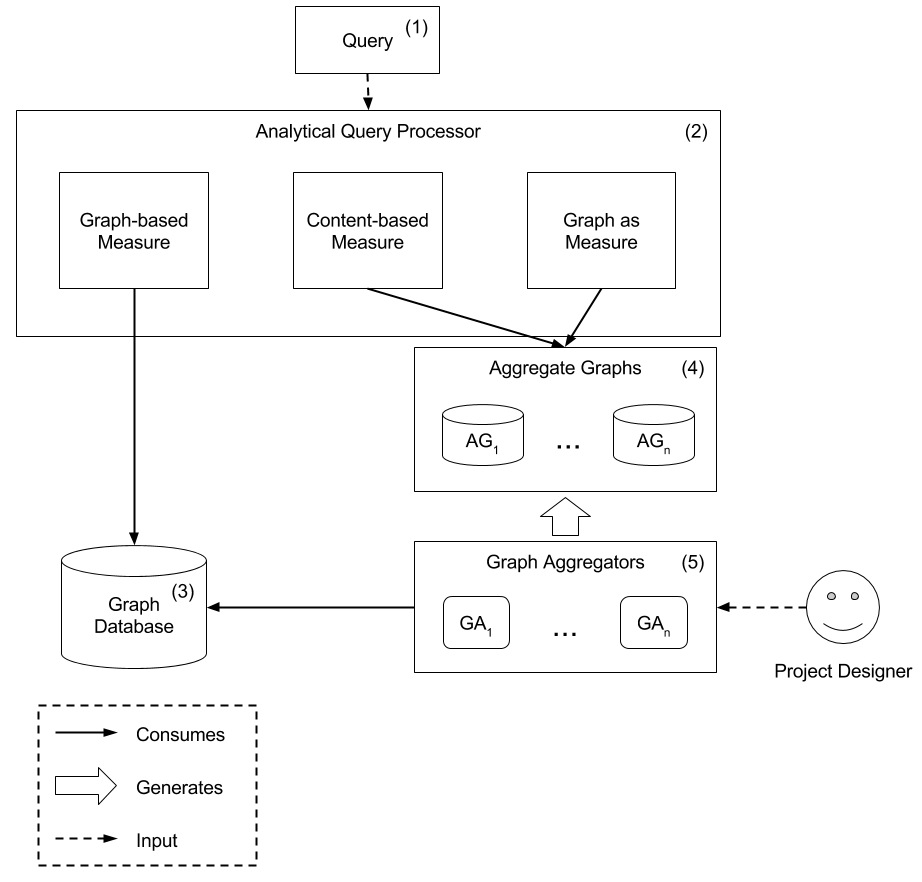
\includegraphics[width=0.8\textwidth]{../Architecture.png}
\caption{OLAP Analysis over Graph Databases Architecture}
\label{fig:figure27}
\end{figure}

The system's input is an analytical query submitted by the user (1), that will be processed by the Analytical Query Processor (AQP) (2). According to the type of measure required by the user, the AQP will determine which specific processor will handle the query: graph-based, content-based or graph measures processors. If the user asks for a graph-based measure, the AQP will consume the original data stored in the graph database (3) to calculate the measure. On the other hand, if the user requires a content-based or a graph as measure, the AQP will calculate the measure based on the data from Aggregate Graphs (4), which are also stored in graph databases.

The Aggregate Graphs are generated by the Graph Aggregators (GAs) (5), which are defined during the design process of the system by the project designer. The project designer is responsible to define what are the dimensions considered in the OLAP system and, therefore, create the GAs that will generate all possible aggregate graphs for the dimensions. More details on Aggregate Graphs and Graph Aggregators are given in the following sections.

The data source considered for this system is a Graph Database that follows the labeled property graph model and supports heterogeneous graphs. This means that vertices can have one or more labels indicating different types of entities. Vertices and edges can have properties. We assume that the data stored in the GDB is integrated, i.e. the data in the repository is consistent, well-formatted and normalised.

\section{Aggregate Graph}
Given a graph $G = (V, E, L_V, L_E, A_V, A_E)$ and a set of dimensions $D = \{d_1, \dots, d_n\}$, where $d_i \in A_V \cup A_E$, an aggregate graph is generated by applying an aggregate function $F$ to one or more dimensions. The result is a new graph $G_A = (V_A, E_A, L_{VA}, L_{EA}, A_{VA}, A_{EA})$, where:
\begin{itemize}
\item $VA = \{v^A_1, \dots, v^A_n\}$ is a set of aggregate vertices, where each vertex $v^A_i$ either (i) corresponds to the result of applying the function $F$ to a set of vertices $V' \subseteq V$ that is associated with a set of attributes $\{a_1, \dots, a_k\}$ containing one or more dimensions in $D$ or (ii) corresponds to a vertex in $V$.
\item $E_A \subseteq V_A \times V_A$ is a set of aggregate edges, where each edge $e^A_i$ either (i) corresponds to the result of combining a set of edges $E' \subseteq E$ that connects one or more vertices in $V$ that were aggregated in $V_A$ or (ii) corresponds to an edge in $E$.
\item $L_{VA}$ is a set of aggregate vertex labels and $L_{EA}$ is a set of aggregate edge labels
\item $A_{VA} = \{a_1, \dots, a_n\}$ is the set of attributes for the aggregate vertices, where $a_i = (k_i, m_i)$ is a key-value pair, $k_i$ is the attribute key and $m_i$ is the attribute value. Each aggregate vertex $v_i \in V_A$ is associated with an attribute vector. $A_{EA} = \{b_1, \dots, b_n\}$ is the set of aggregate edge attributes defined in the same way as aggregate vertices attributes.
\end{itemize}

Consider the graph depicted in Figure \ref{fig:figure26} of our running example. Figure \ref{fig:figure28} shows the aggregate graph $G_A$ obtained by applying the aggregate function COUNT to the dimension set $D = \{d\}$, where $d = (year, Publication)$. Notice that the resulting aggregate graph ends up with the same \emph{Author} vertices as the original graph, since these vertices do not have attributes contained in the dimension set $D$. The \emph{Publication} vertices were aggregated according to their \emph{year} attribute, resulting in three vertices representing the works published in 2017, 2016 and 2015. The aggregate vertices also store the measure calculated using the function COUNT. The edges with the label PUBLISHED were combined, representing the connection between each author and the group of works published in a specific year. The combined edges also store the measure obtained by the use of COUNT function.

\begin{figure}[!h]
\centering
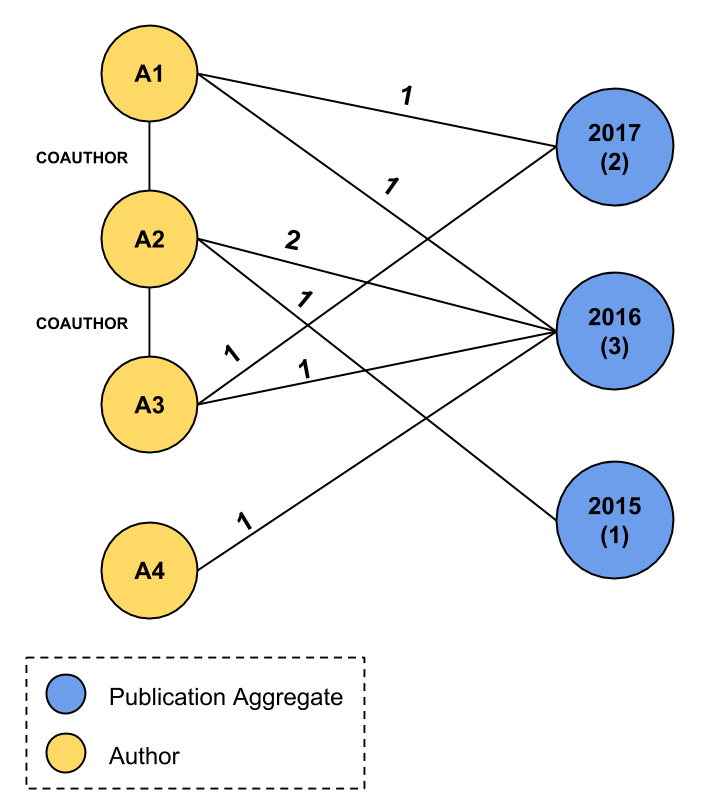
\includegraphics[width=0.4\textwidth]{../aggregate_graph_running_example.png}
\caption{Aggregate Graph obtained from running example graph}
\label{fig:figure28}
\end{figure}

\section{Graph Aggregators}

The Graph Aggregators (GAs) are modules responsible for generating the aggregate graph that will be used to answer the analytical query submitted by the user. During the design process of the system, the Project Designer is responsible for building the GAs based on the dimensions and measures the system should be able to analyse. Each GA will receive as input the original graph G stored in the Graph Database, the set of dimensions to be aggregated D, the aggregate function F and should provide as output an aggregate graph as defined in the previous section. Algorithm \ref{alg:algorithm1} describes the process performed by a GA in order to generate an aggregate graph.

\begin{algorithm}[!h]
 \caption{Graph Aggregator Process}\label{alg:algorithm1}
  \begin{algorithmic}[1]
    \Function{$generateAggGraph$}{$G, F, D$}
      \State $dimValue$ \Comment{set of values for dimensions being aggregated}
      \State $aggVertices$ \Comment{map from dimensions values to set of vertices with corresponding values}  \label{alg:line2}
      \State $aggEdges$ \Comment{map from dimensions values to set of edges with corresponding values} \label{alg:line3} 
      \State $nonAggVertices$ \Comment{set of vertices that were not aggregated}  \label{alg:line31} 
      \State $originalVertices \gets G.vertices$ \Comment{set of vertices from the original graph} \label{alg:line32}
      \ForAll{ $vertex \textrm{ in } originalVertices$}  \label{alg:line4}
        \If {$vertex  \textrm{ in } D$}  \label{alg:line5}
          \State $dimValue \gets getDimValue(vertex, D)$
           \If {$dimValue  \textrm{ in } aggVertices$}  \label{alg:line7}
             \State $aggregateVertices(dimValue, vertex, F)$  \label{alg:line8}
             \State $aggregateEdges(dimValue, vertex, F)$  \label{alg:line9}
           \Else
              \State $aggVertices.add(dimValue, vertex)$  \label{alg:line11}
              \State $aggregateEdges(dimValue, vertex, F)$  \label{alg:line12}
           \EndIf
       \Else 
          \State $nonAggVertices(vertex)$ \Comment{vertex does not contain the dimensions being aggregated}  \label{alg:line15}
        \EndIf
      \EndFor
      \State $aggGraph \gets (aggVertices \cup nonAggVertices, aggEdges)$  \label{alg:line18}
      \State \Return $aggGraph$  \label{alg:line19}
    \EndFunction
  \end{algorithmic}
\end{algorithm}

The GA algorithm starts by creating an empty set of aggregate vertices and edges (lines \ref{alg:line2} and \ref{alg:line3}) that will compose the final aggregate graph that will be returned. Then, the GA will iterate over all the vertices (nodes) of the original graph G (line \ref{alg:line4}), checking for each node if it has the same label as the dimension being aggregated (line \ref{alg:line5}). If the node has the same label, the algorithm checks if already exists an aggregate node for the dimension value of the node (line \ref{alg:line7}). If the aggregate node exists, we collapse the value of the node to the value of the aggregate node using the function F and updating the aggregate node value (line \ref{alg:line8}). We also aggregate the edges that are connected to the node accordingly (line \ref{alg:line9}). If the aggregate node does not exist, we add a new aggregate node with the initial value equals to node's dimension value and aggregate its edges accordingly (lines \ref{alg:line11} and \ref{alg:line12}). If the node does not have the same label as the dimension being aggregated, we only add the node as it is to the non aggregate vertices set (line \ref{alg:line15}). Finally, we setup the aggregate graph and return it (lines \ref{alg:line18} and \ref{alg:line19}).

Once the aggregate graph is generated, it will be stored in a graph database and it will be accessed by the Analytical Query Processor.

\section{Analytical Query Processor}

The Analytical Query Processor (AQP) is responsible for processing the query submitted by the user. The user is responsible for submitting the correct query based on the information he/she is trying to retrieve, i.e. the query should be written according to the type of measure being requested:
\begin{description}
\item[Content-based measure] To calculate this measure, the AQP consumes the data from an aggregate graph and uses the aggregate function to give the resulting measure, which can be a single value, a list or a table of values. This module's response is similar to the response given by traditional OLAP systems.

From our running example, we can ask for the number of publications by year. In this case AQP consumes the data from the aggregate graph illustrated in Figure \ref{fig:figure28} and it would list the nodes with \emph{Publication Aggregate} label, which already contains the count measure as attribute.

\item[Graph-based measure] To calculate this measure, the AQP consumes the data from the original graph database and executes network analysis algorithms on the data. 

In our running example, we could submit a query asking for the \emph{Author} node with highest centrality degree. The AQP calculates the centrality degree for each node in the original graph using an external library. Then, it should return the node with id \textbf{A2}, since it is the Author node with the highest number of connections with other nodes.

\item[Graph as measure] For this type of measure, the AQP also consumes data from an aggregate graph, but in this case, the measure is the aggregated graph itself. Therefore, this module does not need to perform other calculations.

For instance, the aggregate graph shown in Figure \ref{fig:figure28} can be considered a measure if the user requests a topological view of the original data grouping the publications by year.
\end{description}

\section{Final Considerations}
In this chapter, we showed the main components of the proposed system and what is the general operation to answer an analytical query. We also specified in details how each one of the components works and what are their roles in the data analysis process. In the next chapter, we will report how the proposed system was implemented and show some experiments and the results obtained.